\documentclass[12pt]{article} % use larger type; default would be 10pt

\usepackage{pgfplots}
\usetikzlibrary{calc}
\usetikzlibrary{arrows}
\usetikzlibrary{patterns}
\usetikzlibrary{calc,intersections,through,backgrounds}
\usetikzlibrary{decorations.pathreplacing}
        \newcommand\degree[0]{^{\circ}}
        \newcommand\abs[1]{\left|#1\right|}

\title{Play with TikZ}
\author{Just Us}
%\date{} % Activate to display a given date or no date (if empty),
         % otherwise the current date is printed 

\begin{document}
\maketitle

\section{10.1 Polar coordinates }



fig10-1-1a

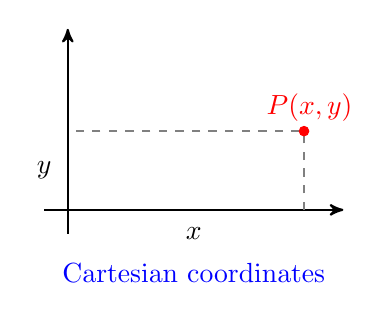
\begin{tikzpicture}
\coordinate (O) at (0,0);
\def\a{3};
\def\b{1};

\coordinate (P) at (\a,\b);
\coordinate (x) at (\a,0);
\coordinate (A) at ({\a+.5},0);
\coordinate (y) at (0,\b);

\draw[black,  thick, ->, >=stealth'] (O)++(-.3,0) --(A);
\draw[black,  thick, ->, >=stealth'] (O)++(0,-.3) -- (0,2.3) ;
\draw[gray, thick, dashed] (x) -- (P) -- (y);

\filldraw[red] (P) circle (1.7pt) node[anchor = south, xshift=2]{$P(x,y)$}; 

\node at (1.6,-.3) {$x$};
\node at (-.3, 0.5) {$y$};
\node at (1.6,-.8)     {\color{blue} Cartesian coordinates};

\end{tikzpicture}
\newline



fig10-1-1b

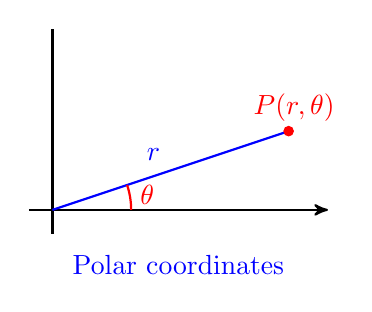
\begin{tikzpicture}
\coordinate (O) at (0,0);
\def\a{3};
\def\b{1};

\coordinate (P) at (\a,\b);
\coordinate (x) at (\a,0);
\coordinate (A) at ({\a+.5},0);
\coordinate (y) at (0,\b);

\draw[black,  thick, ->, >=stealth'] (O)++(-.3,0) --(A);
\draw[black,  thick] (O)++(0,-.3) -- (0,2.3) ;
\draw[blue,  thick] (O) --  ++(P) node[above left, midway,  ]{$r$}  ;

\draw[red, thick] (O)++(1,0) arc (0:{atan(\b /\a)}:1) node [right, midway,xshift=0,yshift=1] {$ \theta$};

\filldraw[red] ($ (O)+(P)$) circle (1.7pt) node[anchor = south, xshift=2]{$P(r, \theta)$}; 
\node at (1.6,-.7)     {\color{blue} Polar coordinates};

\end{tikzpicture}
\newline


fig10-1-2

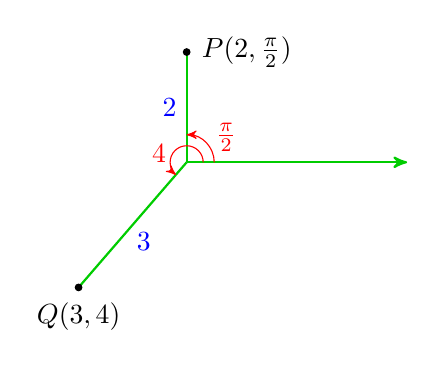
\begin{tikzpicture} [scale=.7]

\coordinate (O) at (0,0);
\coordinate (x) at (4,0);
\coordinate (P) at (90:2);
\coordinate (Q) at ({deg(4)}:3);

\draw[green!80!black, thick, ->, >=stealth'] (O)--(x);
\draw[green!80!black, thick] (O)--(P) node[left, midway, text=blue]{2};
\draw[green!80!black, thick] (O)--(Q) node[below, midway, xshift=4, yshift=1, text=blue]{3};

\filldraw[black] (P) circle (1.7pt) node[anchor = west, xshift=2]{$P(2, \frac{\pi}{2})$}; 
\filldraw[black] (Q) circle (1.7pt) node[anchor = north, yshift=-2]{$Q(3,4)$}; 

\draw[red, ->, >=stealth'] (.5,0) arc(0:90:.5) node[right, midway, yshift=2] {$\frac{\pi}{2}$};

\draw[red, ->, >=stealth'] (.3,0) arc(0:{deg(4)}:.3) node[above left, yshift=1] {4};

\end{tikzpicture}
\newline


fig10-1-3

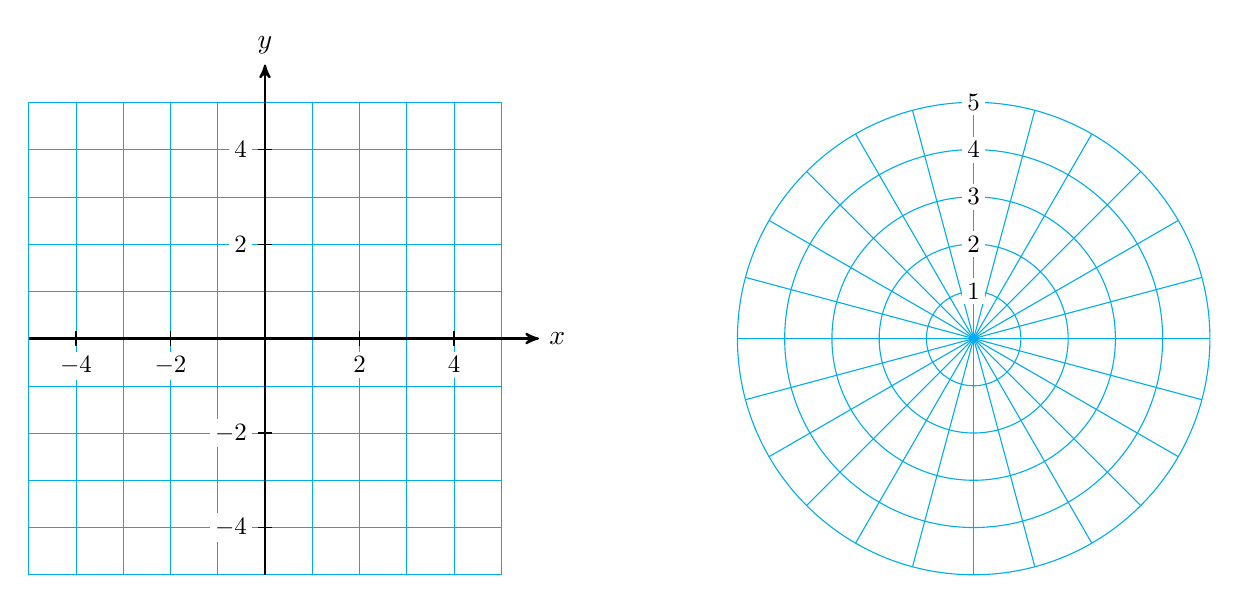
\begin{tikzpicture} [scale=.6]
\def\d{-15};
\draw[step=1cm,cyan,very thin] ({\d-5},-5) grid ({\d+5},5);
\draw[thick,->, >=stealth'] (-20,0) -- ++(10.8,0) node[anchor=west] {$x$};
\draw[thick,->, >=stealth'] (-15,-5) -- ++(0,10.8) node[anchor=south] {$y$};
\foreach \x in {-4,-2,2,4} {
\draw[black] ({\d+\x},.15) -- ++(0,-.3) node[below, yshift=-2, fill=white, inner sep=2, scale=.9]{$\x$};
\draw[black] ({\d+.15},\x) -- ++(-.3,0) node[left, xshift=-2, fill=white, inner sep=2, scale=.9]{$\x$};
}

%polar 
\coordinate(O) at (0,0);
\foreach \angle [count=\xi] in {0, 15, ..., 345}{
  \draw[cyan] (\angle:0) -- (\angle:5);
}
\foreach \r in {1,2,3,4,5} {
\draw[cyan] (O) circle (\r);
\node[fill=white, inner sep = 2, text=black, scale=.9] at (90:\r) {$\r$};
}

\end{tikzpicture}
\newline



exam10-1-1


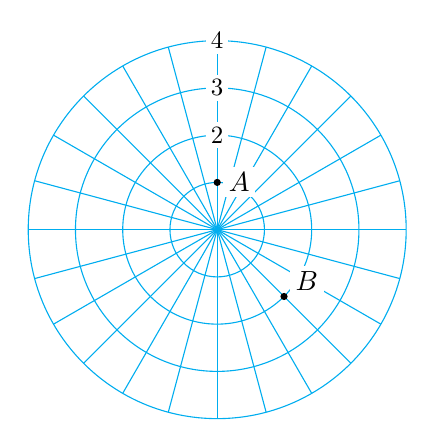
\begin{tikzpicture} [scale=.6]
\coordinate(O) at (0,0);
\coordinate(A) at (90:1);
\coordinate(B) at (315:2);
\foreach \angle [count=\xi] in {0, 15, ..., 345}{
  \draw[cyan] (\angle:0) -- (\angle:4);
}
\draw[cyan] (O) circle (1);
\foreach \r in {2,3,4} {
\draw[cyan] (O) circle (\r);
\node[fill=white, inner sep = 2, text=black, scale=.9] at (90:\r) {$\r$};
}
\filldraw[black] (A) circle (1.8pt) node[anchor = west, xshift=2, fill=white, inner sep=2]{$A$}; 
\filldraw[black] (B) circle (1.8pt) node[anchor = south west, xshift=2, fill=white, inner sep=2]{$B$}; 

\end{tikzpicture}
\newline



exer10-1-1


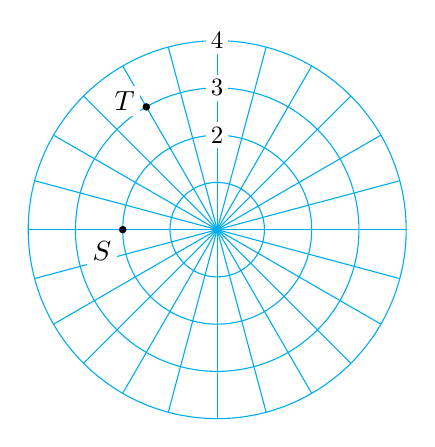
\begin{tikzpicture} [scale=.6]
\coordinate(O) at (0,0);
\coordinate(T) at (120:3);
\coordinate(S) at (180:2);
\foreach \angle [count=\xi] in {0, 15, ..., 345}{
  \draw[cyan] (\angle:0) -- (\angle:4);
}
\draw[cyan] (O) circle (1);
\foreach \r in {2,3,4} {
\draw[cyan] (O) circle (\r);
\node[fill=white, inner sep = 2, text=black, scale=.9] at (90:\r) {$\r$};
}
\filldraw[black] (T) circle (1.9pt) node[anchor = east, xshift=-2, yshift=2, fill=white, inner sep=2]{$T$}; 
\filldraw[black] (S) circle (1.9pt) node[anchor = north east, xshift=-2, yshift=-2, fill=white, inner sep=2]{$S$}; 

\end{tikzpicture}
\newline



fig10-1-4


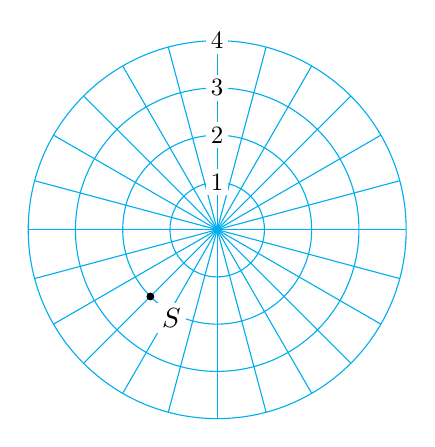
\begin{tikzpicture} [scale=.6]
\coordinate(O) at (0,0);
\coordinate(Q) at (225:2);
\foreach \angle [count=\xi] in {0, 15, ..., 345}{
  \draw[cyan] (\angle:0) -- (\angle:4);
}
\foreach \r in {1,2,3,4} {
\draw[cyan] (O) circle (\r);
\node[fill=white, inner sep = 2, text=black, scale=.9] at (90:\r) {$\r$};
}
\filldraw[black] (Q) circle (2pt) node[anchor = north west, xshift=2, yshift=-2, fill=white, inner sep=2]{$S$}; 

\end{tikzpicture}
\newline




fig10-1-5

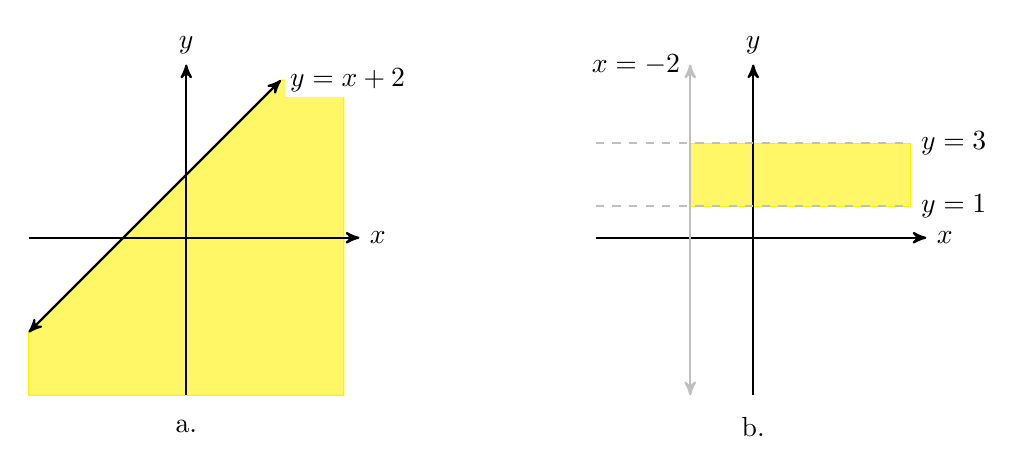
\begin{tikzpicture} [scale=.4]
\draw[fill=yellow, yellow, fill opacity = 0.6,] (-5,-5)--(-5,-3)--(3,5)--(5,5)--(5,-5)--(-5,-5);

\draw[black, thick, ->, >=stealth'] (-5,0)--(5.5,0)node[right] {$x$};
\draw[black, thick, ->, >=stealth'] (0,-5)--(0,5.5)node[above] {$y$};

\draw[black, thick, <->, >=stealth'] (-5, -3)--(3,5)node[right, fill=white, inner sep=2, xshift=1] {$y=x+2$};
\node at (0,-6){a.};

%second grid
\coordinate(O) at (18,0);
\draw[fill=yellow, yellow, fill opacity = 0.6,] (O)++(-2,3)--++(7,0)--++(0,-2)--++(-7,0)--++(0,2);

\draw[black, thick, ->, >=stealth'] (O)++(-5,0)--++(10.5,0)node[right] {$x$};
\draw[black, thick, ->, >=stealth'] (O)++(0,-5)--++(0,10.5)node[above] {$y$};
\draw[lightgray, thick, dashed] (O)++(-5,1)--++(10,0 )node[right, text=black] {$y=1$};
\draw[lightgray, thick, dashed] (O)++(-5,3)--++(10,0 )node[right, text=black] {$y=3$};
\draw[lightgray, thick, <->, >=stealth'] (O)++(-2,-5)--++(0,10.5 ) node[left, text=black] {$x=-2$};
\node at ($(O)+(0,-6)$){b.};

\end{tikzpicture}
\newline


exam10-1-3

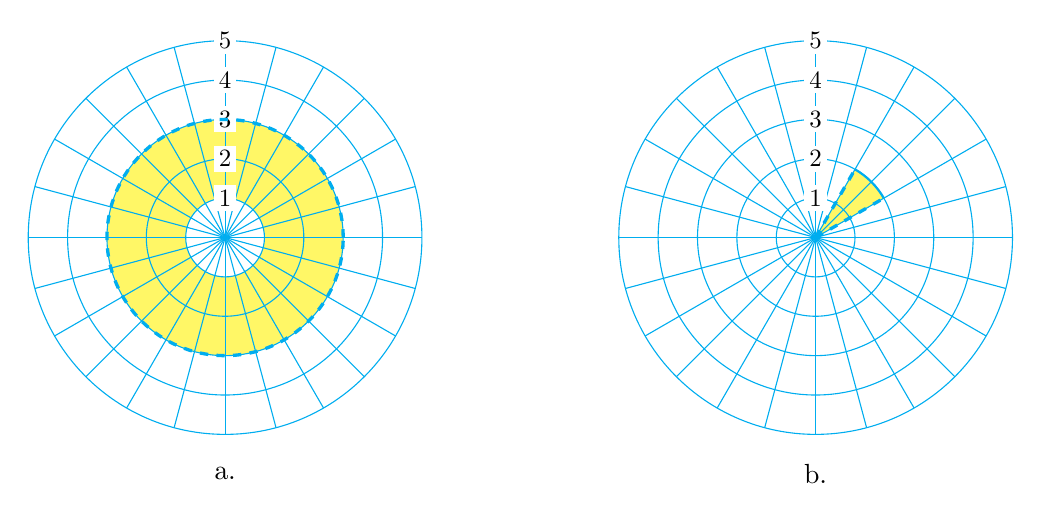
\begin{tikzpicture} [scale=.5]
\coordinate(O) at (0,0);
\path [draw=none,fill=yellow, fill opacity = 0.6,even odd rule] (O) circle (1) (O) circle (3);
\foreach \angle [count=\xi] in {0, 15, ..., 345}{
  \draw[cyan] (\angle:0) -- (\angle:5);
}
\foreach \r in {1,2,3,4,5} {
\draw[cyan] (O) circle (\r);
\node[fill=white, inner sep = 2, text=black, scale=.9] at (90:\r) {$\r$};
}
\draw[cyan, very thick,dashed] (O) circle (3);

\node at (0,-6){a.};

%second grid
\coordinate(O) at (15,0);
\path [draw=none,fill=yellow, fill opacity = 0.6] (O)--++(30:2) arc(30:60:2) -- ++(240:2);
\foreach \angle [count=\xi] in {0, 15, ..., 345}{
  \draw[cyan] (O)++(\angle:0) -- ++(\angle:5);
}
\foreach \r in {1,2,3,4,5} {
\draw[cyan] (O) circle (\r);
\node[fill=white, inner sep = 2, text=black, scale=.9] at ($ (O)+(90:\r)$) {$\r$};
}
\draw[cyan, very thick,dashed] (O)--++(30:2);
\draw[cyan, very thick,dashed] (O)--++(60:2);
\draw[cyan, thick] (O)++(60:2) arc(60:30:2);
\node at ($(O)+(0,-6)$){b.};

\end{tikzpicture}
\newline


exer10-1-3

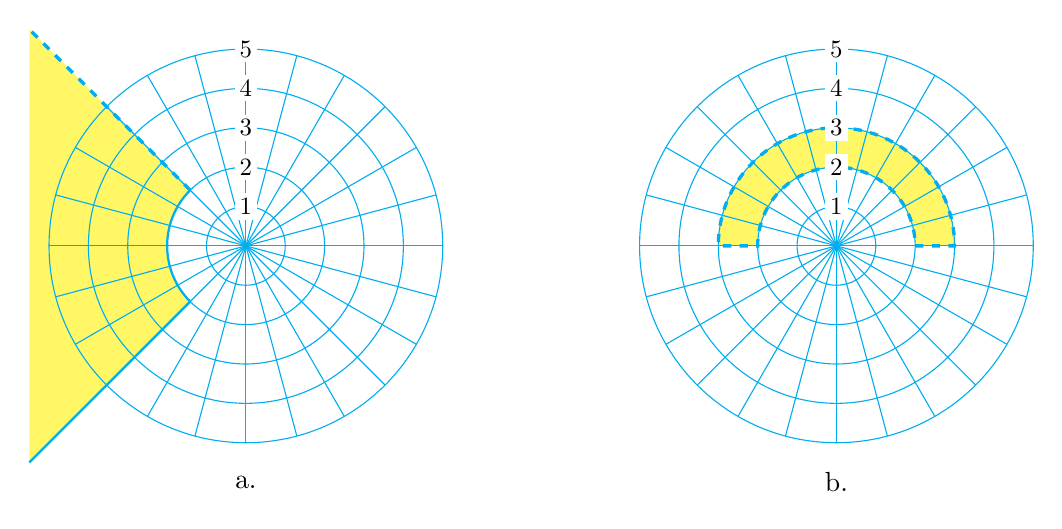
\begin{tikzpicture} [scale=.5]
\coordinate(O) at (0,0);
\path [draw=none,fill=yellow, fill opacity = 0.6] (135:2)--(135:{5.5*sqrt(2)}) -- (225:{5.5*sqrt(2)})--(225:2) arc(225:135:2);
\foreach \angle [count=\xi] in {0, 15, ..., 345}{
  \draw[cyan] (\angle:0) -- (\angle:5);
}
\foreach \r in {1,2,3,4,5} {
\draw[cyan] (O) circle (\r);
\node[fill=white, inner sep = 2, text=black, scale=.9] at (90:\r) {$\r$};
}
\draw[cyan, very thick,dashed] (135:2)--(135:{5.5*sqrt(2)});
\draw[cyan,  thick] (225:2)--(225:{5.5*sqrt(2)});
\draw[cyan,  thick] (225:2) arc(225:135:2);
\node at (0,-6){a.};

%second grid
\coordinate(O) at (15,0);
\path [draw=cyan,very thick, dashed,fill=yellow, fill opacity = 0.6] (O)++(0:2) --++(0:1) arc(0:180:3) --++(0:1) arc(180:0:2);
\foreach \angle [count=\xi] in {0, 15, ..., 345}{
  \draw[cyan] (O)++(\angle:0) -- ++(\angle:5);
}
\foreach \r in {1,2,3,4,5} {
\draw[cyan] (O) circle (\r);
\node[fill=white, inner sep = 2, text=black, scale=.9] at ($ (O)+(90:\r)$) {$\r$};
}
\node at ($(O)+(0,-6)$){b.};

\end{tikzpicture}
\newline


fig10-1-6

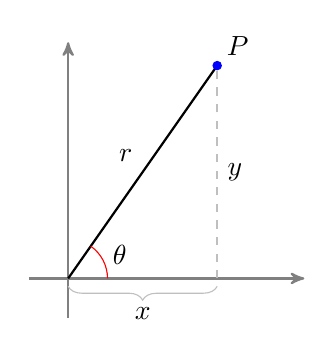
\begin{tikzpicture}
\def\r{3.3};
\def\t{55};
\coordinate(O) at (0,0);
\coordinate(P) at (\t:\r);
\coordinate(x) at (0:{\r*cos(\t)});
\draw[gray,thick,->,>=stealth'] (-0.5,0)--(3,0);
\draw[gray,thick,->,>=stealth'] (0, -0.5)--(0,3);
\draw[black,thick] (O)--(P) node[above left, midway]{$r$};
\draw[lightgray,thick, dashed, text=black] (x)--(P) node[right, midway]{$y$};
\draw[red] (0:.5) arc(0:\t:0.5) node[right,midway, yshift=2,text=black] {$\theta$};
\filldraw[blue] (P) circle (1.5pt) node[above right, text=black]{$P$};
\draw [lightgray,decorate,decoration={brace,amplitude=5pt}] (x)++(0, -.1) -- (0,-.1) node [black, below,midway,yshift=-4pt] {$x$};

\end{tikzpicture}
\newline


exam10-1-4 

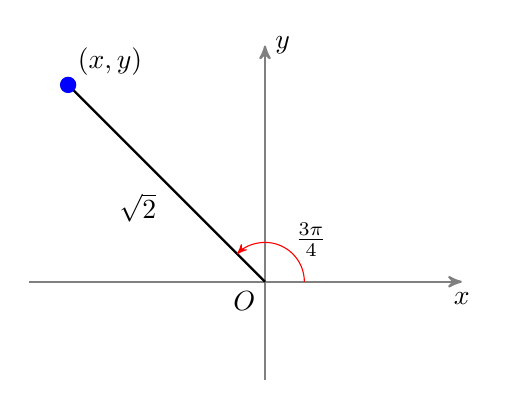
\begin{tikzpicture}  [scale=2.5]
\coordinate(O) at (0,0);
\coordinate(P) at (135:{sqrt(2)});
\draw[gray,thick,->,>=stealth'] (-1.2,0)--(1.,0) node[below, text=black]{$x$};
\draw[gray,thick,->,>=stealth'] (0, -0.5)--(0,1.2) node[right, text=black]{$y$};
\draw[black,thick] (O)--(P) node[below left, midway]{$\sqrt{2}$};
\draw[red, ->,>=stealth'] (0:.2) arc(0:135:0.2) node[right,midway, xshift=2, yshift=2,text=black] {$\frac{3\pi}{4}$};
\filldraw[blue] (P) circle (1.1pt) node[above right, text=black]{$(x,y)$};
\node[below left] at (O) {$O$};
\end{tikzpicture}
\newline


exam10-1-5

\begin{tikzpicture}  [scale=2.5]
\coordinate(O) at (0,0);
\coordinate(P) at (240:1);
\draw[gray,thick,->,>=stealth'] (-1,0)--(1.,0) node[below, text=black]{$x$};
\draw[gray,thick,->,>=stealth'] (0, -1.2)--(0,.8) node[left, text=black]{$y$};
\draw[black,thick] (O)--(P);
\filldraw[blue] (P) circle (1pt) node[below , text=black]{$(-\frac{1}{2},-\frac{\sqrt{3}}{2})$};
\node[below right] at (O) {$O$};
\end{tikzpicture}
\newline

hp10-1-1 polar grid

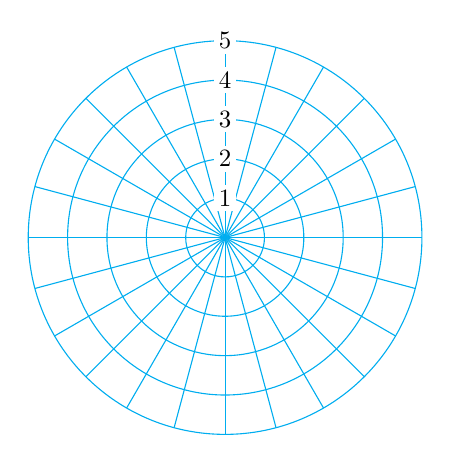
\begin{tikzpicture} [scale=.5]
\coordinate(O) at (0,0);
\foreach \angle [count=\xi] in {0, 15, ..., 345}{
  \draw[cyan] (\angle:0) -- (\angle:5);
}
\foreach \r in {1,2,3,4,5} {
\draw[cyan] (O) circle (\r);
\node[fill=white, inner sep = 2, text=black, scale=.9] at (90:\r) {$\r$};
}

\end{tikzpicture}
\newline


hp10-1-1ans polar grid

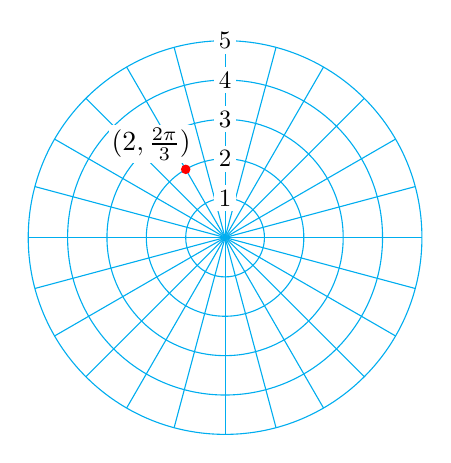
\begin{tikzpicture} [scale=.5]
\coordinate(O) at (0,0);
\foreach \angle [count=\xi] in {0, 15, ..., 345}{
  \draw[cyan] (\angle:0) -- (\angle:5);
}
\foreach \r in {1,2,3,4,5} {
\draw[cyan] (O) circle (\r);
\node[fill=white, inner sep = 2, text=black, scale=.9] at (90:\r) {$\r$};
}

\filldraw[red] (120:2) circle (3pt) node[above left, xshift=3, yshift=2, text=black, fill=white, inner sep=1]{$(2,\frac{2\pi}{3})$};

\end{tikzpicture}
\newline


hp10-1-3ans polar grid

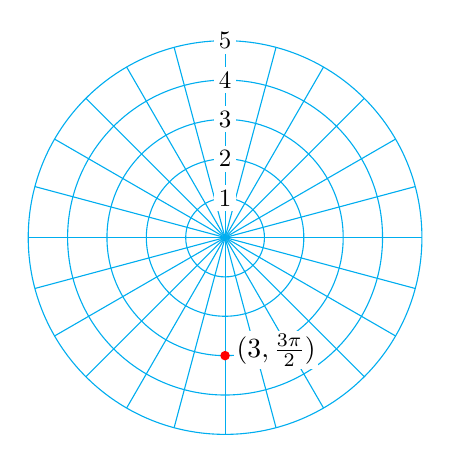
\begin{tikzpicture} [scale=.5]
\coordinate(O) at (0,0);
\foreach \angle [count=\xi] in {0, 15, ..., 345}{
  \draw[cyan] (\angle:0) -- (\angle:5);
}
\foreach \r in {1,2,3,4,5} {
\draw[cyan] (O) circle (\r);
\node[fill=white, inner sep = 2, text=black, scale=.9] at (90:\r) {$\r$};
}

\filldraw[red] (270:3) circle (3pt) node[ right, xshift=3, yshift=2, text=black, fill=white, inner sep=1]{$(3,\frac{3\pi}{2})$};

\end{tikzpicture}
\newline


hp10-1-5ans polar grid

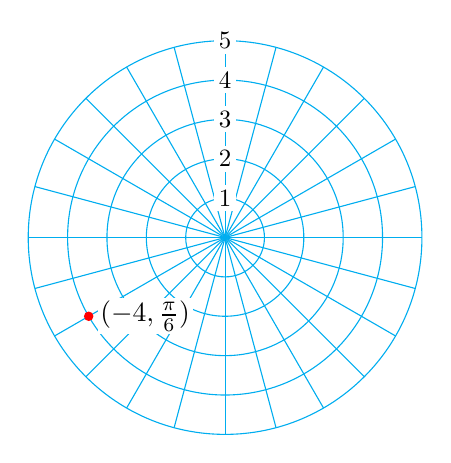
\begin{tikzpicture} [scale=.5]
\coordinate(O) at (0,0);
\foreach \angle [count=\xi] in {0, 15, ..., 345}{
  \draw[cyan] (\angle:0) -- (\angle:5);
}
\foreach \r in {1,2,3,4,5} {
\draw[cyan] (O) circle (\r);
\node[fill=white, inner sep = 2, text=black, scale=.9] at (90:\r) {$\r$};
}

\filldraw[red] (210:4) circle (3pt) node[ right, xshift=3, text=black, fill=white, inner sep=1]{$(-4,\frac{\pi}{6})$};

\end{tikzpicture}
\newline


hp10-1-7ans polar grid

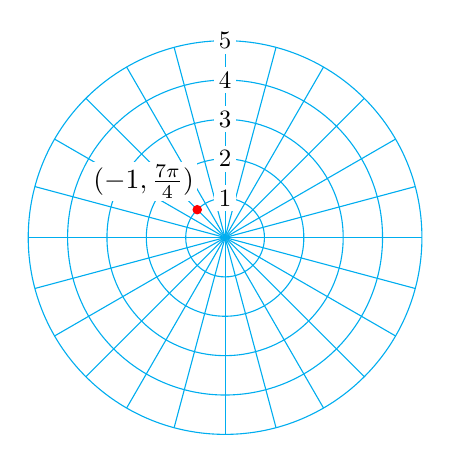
\begin{tikzpicture} [scale=.5]
\coordinate(O) at (0,0);
\foreach \angle [count=\xi] in {0, 15, ..., 345}{
  \draw[cyan] (\angle:0) -- (\angle:5);
}
\foreach \r in {1,2,3,4,5} {
\draw[cyan] (O) circle (\r);
\node[fill=white, inner sep = 2, text=black, scale=.9] at (90:\r) {$\r$};
}

\filldraw[red] (135:1) circle (3pt) node[above left, yshift=3, text=black, fill=white, inner sep=1]{$(-1,\frac{7\pi}{4})$};

\end{tikzpicture}
\newline


hp10-1-9 polar grid

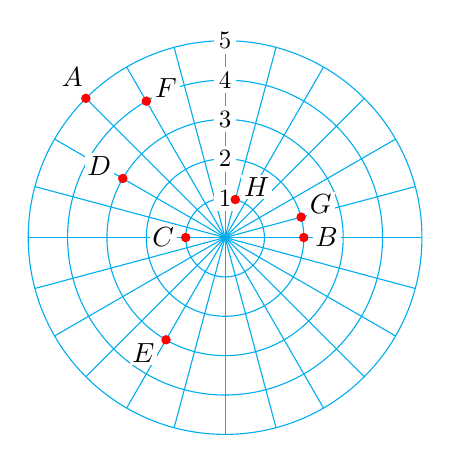
\begin{tikzpicture} [scale=.5]
\coordinate(O) at (0,0);
\foreach \angle [count=\xi] in {0, 15, ..., 345}{
  \draw[cyan] (\angle:0) -- (\angle:5);
}
\foreach \r in {1,2,3,4,5} {
\draw[cyan] (O) circle (\r);
\node[fill=white, inner sep = 2, text=black, scale=.9] at (90:\r) {$\r$};
}
\filldraw[red] (135:5) circle (3pt) node[above left, yshift=3, text=black, fill=white, inner sep=1]{$A$};
\filldraw[red] (0:2) circle (3pt) node[right, xshift=3, text=black, fill=white, inner sep=1]{$B$};
\filldraw[red] (180:1) circle (3pt) node[left, xshift=-3, text=black, fill=white, inner sep=1]{$C$};
\filldraw[red] (150:3) circle (3pt) node[above left, xshift=-3, text=black, fill=white, inner sep=1]{$D$};
\filldraw[red] (240:3) circle (3pt) node[below left, xshift=-3, text=black, fill=white, inner sep=1]{$E$};
\filldraw[red] (120:4) circle (3pt) node[above right, xshift=2, text=black, fill=white, inner sep=1]{$F$};
\filldraw[red] (15:2) circle (3pt) node[above right, xshift=2, text=black, fill=white, inner sep=1]{$G$};
\filldraw[red] (75:1) circle (3pt) node[above right, xshift=2, text=black, fill=white, inner sep=1]{$H$};

\end{tikzpicture}
\newline


hp10-1-39ans polar grid

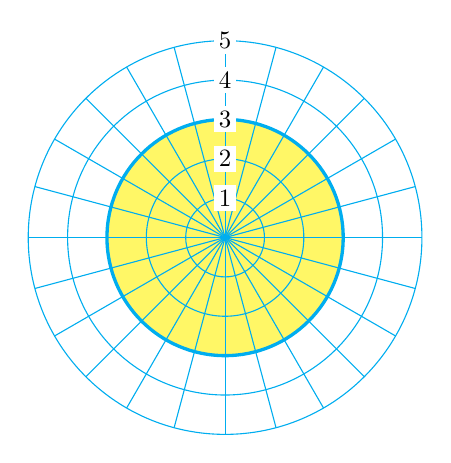
\begin{tikzpicture} [scale=.5]
\coordinate(O) at (0,0);
\draw [draw=none,fill=yellow, fill opacity = 0.6] (O) circle (3);
\draw[cyan, very thick] (O) circle (3);

\foreach \angle [count=\xi] in {0, 15, ..., 345}{
  \draw[cyan] (\angle:0) -- (\angle:5);
}
\foreach \r in {1,2,3,4,5} {
\draw[cyan] (O) circle (\r);
\node[fill=white, inner sep = 2, text=black, scale=.9] at (90:\r) {$\r$};
}

\end{tikzpicture}
\newline


hp10-1-41ans polar grid

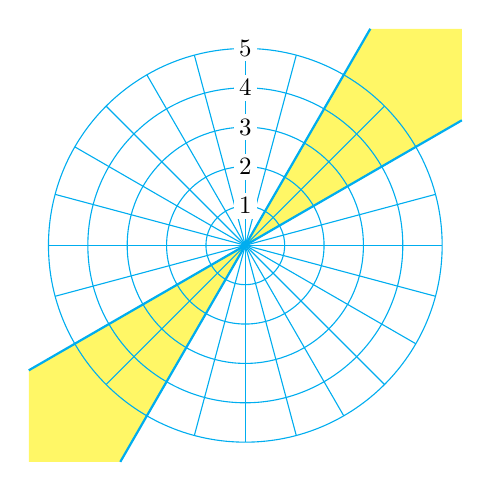
\begin{tikzpicture} [scale=.5]
\coordinate(O) at (0,0);
\path [draw=none,fill=yellow, fill opacity = 0.6] (O)--(30:{11/sqrt(3)}) -- (5.5,5.5)--(60:{11/sqrt(3)}) (O);
\draw[cyan, thick] (60:{11/sqrt(3)})--(O)--(30:{11/sqrt(3)});
\path [draw=none,fill=yellow, fill opacity = 0.6] (O)--(210:{11/sqrt(3)}) -- (-5.5,-5.5)--(240:{11/sqrt(3)}) (O);
\draw[cyan, thick] (210:{11/sqrt(3)})--(O)--(240:{11/sqrt(3)});

\foreach \angle [count=\xi] in {0, 15, ..., 345}{
  \draw[cyan] (\angle:0) -- (\angle:5);
}
\foreach \r in {1,2,3,4,5} {
\draw[cyan] (O) circle (\r);
\node[fill=white, inner sep = 2, text=black, scale=.9] at (90:\r) {$\r$};
}

\end{tikzpicture}
\newline


hp10-1-43ans polar grid

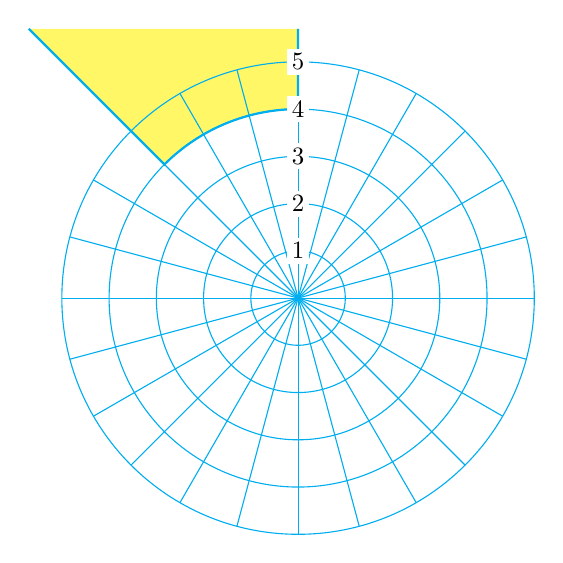
\begin{tikzpicture} [scale=.6]
\coordinate(O) at (0,0);
\path [draw=none,fill=yellow, fill opacity = 0.6] (90:4)--(90:5.7) -- (-5.7,5.7)--(135:4) arc (135:90:4);
\draw[cyan, thick] (90:5.7)--(90:4) arc(90:135:4)--(-5.7,5.7);

\foreach \angle [count=\xi] in {0, 15, ..., 345}{
  \draw[cyan] (\angle:0) -- (\angle:5);
}
\foreach \r in {1,2,3,4,5} {
\draw[cyan] (O) circle (\r);
\node[fill=white, inner sep = 2, text=black, scale=.9] at (90:\r) {$\r$};
}

\end{tikzpicture}
\newline


hp10-1-45 polar region

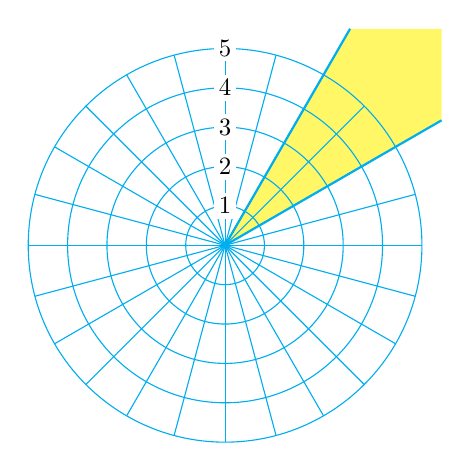
\begin{tikzpicture} [scale=.5]
\coordinate(O) at (0,0);
\path [draw=none,fill=yellow, fill opacity = 0.6] (O)--(30:{11/sqrt(3)}) -- (5.5,5.5)--(60:{11/sqrt(3)}) (O);
\draw[cyan, thick] (60:{11/sqrt(3)})--(O)--(30:{11/sqrt(3)});

\foreach \angle [count=\xi] in {0, 15, ..., 345}{
  \draw[cyan] (\angle:0) -- (\angle:5);
}
\foreach \r in {1,2,3,4,5} {
\draw[cyan] (O) circle (\r);
\node[fill=white, inner sep = 2, text=black, scale=.9] at (90:\r) {$\r$};
}

\end{tikzpicture}
\newline


hp10-1-47 polar region

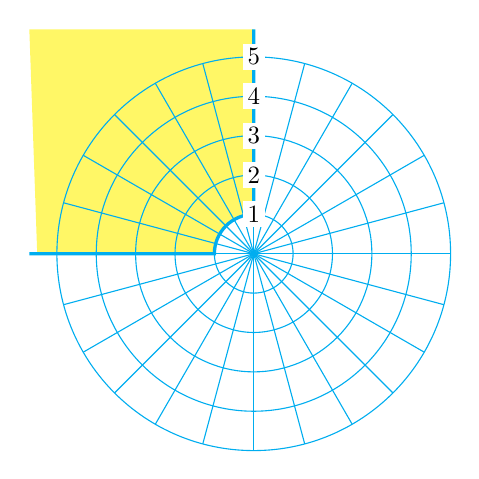
\begin{tikzpicture} [scale=.5]
\coordinate(O) at (0,0);
\path [draw=none,fill=yellow, fill opacity = 0.6] (90:1)--(90:5.7) -- (-5.7,5.7)--(-5.5,0) --(-1,0) arc(180:90:1);
\draw[cyan, very thick] (0,5.7)--(0,1) arc(90:180:1)--(-5.7,0);

\foreach \angle [count=\xi] in {0, 15, ..., 345}{
  \draw[cyan] (\angle:0) -- (\angle:5);
}
\foreach \r in {1,2,3,4,5} {
\draw[cyan] (O) circle (\r);
\node[fill=white, inner sep = 2, text=black, scale=.9] at (90:\r) {$\r$};
}

\end{tikzpicture}
\newline


hp10-1-48 polar region

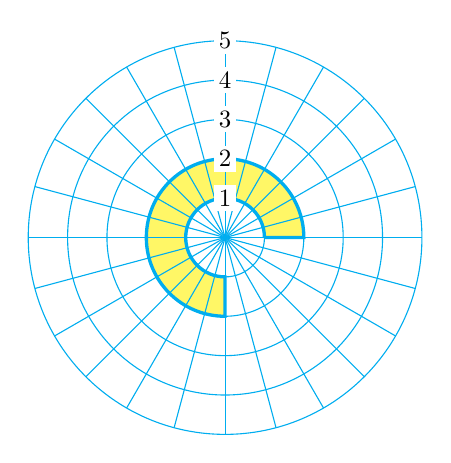
\begin{tikzpicture} [scale=.5]
\coordinate(O) at (0,0);
\path [draw=cyan, very thick,fill=yellow, fill opacity = 0.6] (0:1)--(0:2)   arc(0:270:2) -- (0,-1) arc(270:0:1);

\foreach \angle [count=\xi] in {0, 15, ..., 345}{
  \draw[cyan] (\angle:0) -- (\angle:5);
}
\foreach \r in {1,2,3,4,5} {
\draw[cyan] (O) circle (\r);
\node[fill=white, inner sep = 2, text=black, scale=.9] at (90:\r) {$\r$};
}

\end{tikzpicture}
\newline


hp10-1-49 polar region

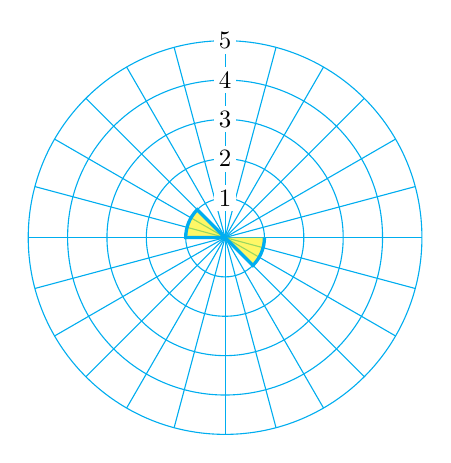
\begin{tikzpicture} [scale=.5]
\coordinate(O) at (0,0);

\foreach \angle [count=\xi] in {0, 15, ..., 345}{
  \draw[cyan] (\angle:0) -- (\angle:5);
}
\foreach \r in {1,2,3,4,5} {
\draw[cyan] (O) circle (\r);
\node[fill=white, inner sep = 2, text=black, scale=.9] at (90:\r) {$\r$};
}
\path [draw=cyan, very thick,fill=yellow, fill opacity = 0.6] (O)--(135:1)   arc(135:180:1) -- (O)--(-45:1) arc(-45:0:1);

\end{tikzpicture}
\newline


hp10-1-50 polar region

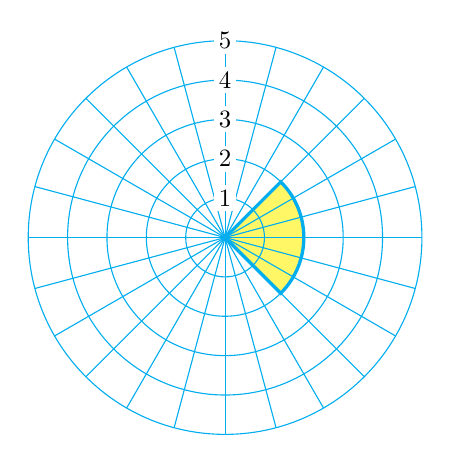
\begin{tikzpicture} [scale=.5]
\coordinate(O) at (0,0);
\path [draw=cyan, very thick,fill=yellow, fill opacity = 0.6] (O)--(-45:2)   arc(-45:45:2) -- (O);

\foreach \angle [count=\xi] in {0, 15, ..., 345}{
  \draw[cyan] (\angle:0) -- (\angle:5);
}
\foreach \r in {1,2,3,4,5} {
\draw[cyan] (O) circle (\r);
\node[fill=white, inner sep = 2, text=black, scale=.9] at (90:\r) {$\r$};
}

\end{tikzpicture}
\newline





\end{document}
